\renewcommand{\lsql}[1]{\lstinline[language=SQL,prebreak=]!#1!}

\lab{Python}{Advanced SQL}{SQL II}
\objective{Learn more of the advanced and specialized features of SQL.}
\label{lab:advancedsql}

\section*{Database Normalization}
Normalizing a database is the process of organizing tables and columns to minimize the amount of redundant information in the database.
For example, a non-normalized database might have a table that stores customer contact information and a table that contains all of the products a company has sold.
However, they want want to track who buys what products in case they need to contact them later, and to do so, they store all the contact information of particular buyer along with the every item they purchased.
Now, two tables store the customer contact information.
If we needed to update a customer's phone number, we have to update two tables.
While that may not be bad for small databases, larger databases would be near impossible to update correctly.
The idea of normalizing a database allows us to store all customer contact information in one place in the database.
All other tables that might need a customer's name, phone number, or address would reference the contact information table.
When an update needs to be performed, we only need to update the contact information table.
Then any table that references this information is also automatically up to date.

To properly normalize a database, we need to discuss the types of relations tables might have.
\subsection*{One to One}
This is the simplest relation to model.
A single table can be used to express this relation.
The relation is between one record and at most one other record.
An example of this relationship is an employee and their organization.
One employee works at one organization.
Another example would be a driver's license belongs to only one person.

\subsection*{One to Many}
This relationship and it inverse must be modeled with at least two tables.
The general approach is to use a unique ID.
Note that a relationship that appears one to one may actually be a one to many relationship.
Many people will, therefore, use the same unique ID approach on one to one relationships too in the case it turns out to be a one to many relationship.
An example of a one to many relationship would between an department and its employees.
The department would receive a unique ID and then each employee in that department would be tagged with that ID.

\subsection*{Many to Many}
This relationship requires at least three tables.
A many to many relationship can be visualized as two, separate one to many relationships.
The records in each of the two tables receive a unique ID.
A third table then serves as a map between IDs of table to IDs of the other table.
And example of a many to many relationship is doctors and patients.
One doctor can have several patients and one patient can have several doctors.

For the rest of the lab, we will be using tables: \ref{table:students}, \ref{table:majors}, \ref{table:grades}, and \ref{table:classes}.

\begin{table}
\begin{tabular}{|l|l|l|}
\hline
StudentID & Name & MajorCode \\
\hline
401767594 & Michelle Fernandez & 1 \\
678665086 & Gilbert Chapman & NULL \\
553725811 & Roberta Cook & 2 \\
886308195 & Rene Cross & 3 \\
103066521 & Cameron Kim & 4 \\
821568627 & Mercedes Hall & NULL \\
206208438 & Kristopher Tran & 2 \\
341324754 & Cassandra Holland & 1 \\
262019426 & Alfonso Phelps & NULL \\
622665098 & Sammy Burke &2 \\
\hline
\end{tabular}
\caption{students}
\label{table:students}
\end{table}

\begin{table}
\begin{tabular}{|l|l|}
\hline
ID & Name \\
\hline
1 & Math \\
2 & Science \\
3 & Writing \\
4 & Art \\
\hline
\end{tabular}
\caption{majors}
\label{table:majors}
\end{table}

\begin{table}
\begin{tabular}{|l|l|l|}
\hline
StudentID & ClassID & Grade \\
\hline
401767594 & 4 & C \\
401767594 & 3 & B- \\
678665086 & 4 & NULL \\
678665086 & 3 & A+ \\
553725811 & 2 & C \\
678665086 & 1 & NULL \\
886308195 & 1 & A \\
103066521 & 2 & C \\
103066521 & 3 & C- \\
821568627 & 4 & D \\
821568627 & 2 & NULL \\
821568627 & 1 & B \\
206208438 & 2 & A \\
206208438 & 1 & C+ \\
341324754 & 2 & D- \\
341324754 & 1 & NULL \\
103066521 & 4 & A \\
262019426 & 2 & B \\
262019426 & 3 & NULL \\
622665098 & 1 & A \\
622665098 & 2 & A- \\
\hline
\end{tabular}
\caption{grades}
\label{table:grades}
\end{table}

\begin{table}
\begin{tabular}{|l|l|}
\hline
ClassID & Name \\
\hline
1 & Calculus \\
2 & English \\
3 & Pottery \\
4 & History \\
\hline
\end{tabular}
\caption{classes}
\label{table:classes}
\end{table}

\begin{problem}
Classify the relations between the various records in these tables: \ref{table:students}, \ref{table:majors}, \ref{table:grades}, and \ref{table:classes}.

Classify each relation as either one to one, one to many, or many to many.
Identify the tables used in each relationship.
\end{problem}

\begin{info}
There are instances where you would not want a completely normalized database.
Whether to normalize your database depends on your specific needs.
Usually, though, the decision to denormalize a database is a last-resort attempt to improve performance.
\end{info}

\section*{Joining tables}
We can use SQL to join two or more tables together for a query.
This is a very powerful tool.
SQLite supports three types of standard table joins.

Joining tables is a common practice to collect data from different parts of the database into a single table.
Joins are absolutely essential in a normalized database since data is split between multiple tables.

\subsection*{Inner Join}
This is often the default join operation in SQL.
An inner join can be depicted as an intersection of two or more tables.
\begin{figure}
\centering
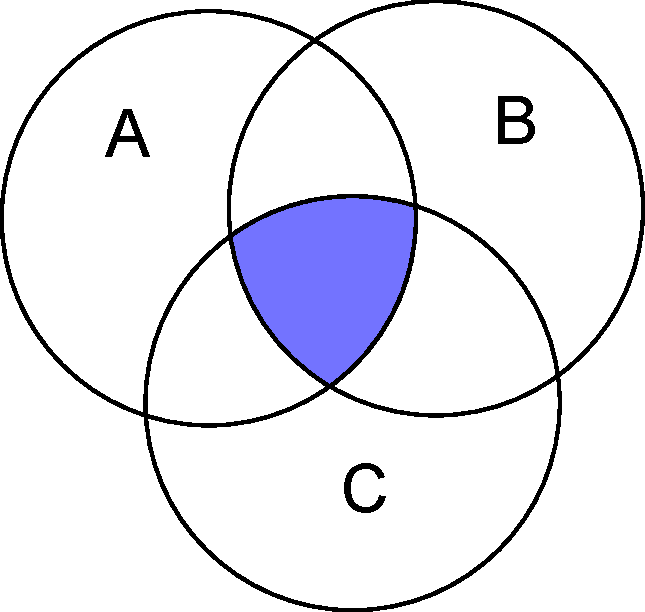
\includegraphics[width=.5\textwidth]{inner_join.pdf}
\caption{An inner joining of tables A, B, and C.}
\label{fig:inner_join}
\end{figure}
When performing an inner join on tables, the result will only be those records that match across all tables.
\begin{lstlisting}[language=SQL]
SELECT students.name, majors.name FROM students JOIN majors ON students.majorcode=majors.id;
\end{lstlisting}
An inner join is equivalent to the following pseudo-loop in Python
\begin{lstlisting}
for row_s in students:
    for row_m in majors:
        if predicates(row_s, row_m):
            yield columns
\end{lstlisting}

\begin{table}
\begin{tabular}{|l|l|}
\hline
students.name & majors.name \\
\hline
Michelle Fernandez & Math \\
Roberta Cook & Science \\
Rene Cross & Writing \\
Cameron Kim & Art \\
Kristopher Tran & Science \\
Cassandra Holland & Math \\
Sammy Burke & Science \\
\hline
\end{tabular}
\caption{An inner join of students and majors}
\label{table:ij_studentsmajors}
\end{table}

\subsection*{Left Outer Join}

\begin{figure}
\centering
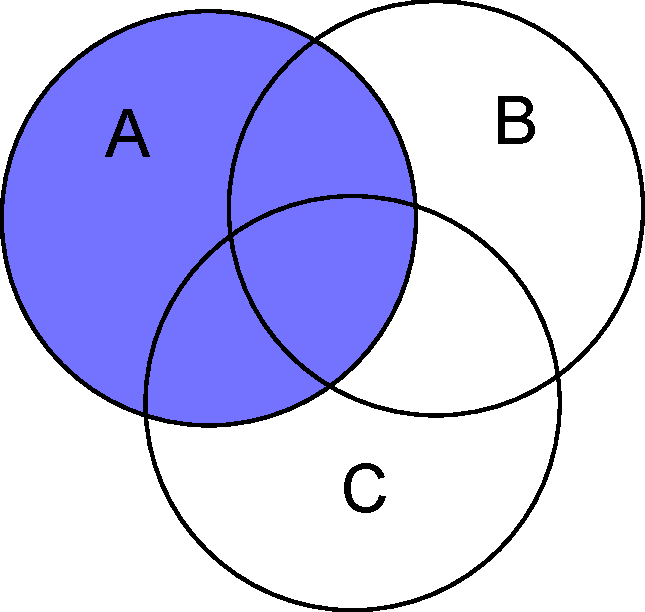
\includegraphics[width=.5\textwidth]{left_outer.pdf}
\caption{A left outer table join of A with tables B and C.}
\label{fig:left_outer}
\end{figure}




\subsection*{Cross Join}
Essentially a cartesian product of tables.  Care must be taken when using cross join because of the size of the joined table.



\section*{Aggregating Functions}
Aggregate functions are useful for summarizing the data in a column.
The functions are
\begin{table}
\begin{tabular}{|l|l|}
\hline
Function & Description \\
\hline
MIN & Retrieve the smallest numeric value of a column \\
MAX & Retrieve the largest numeric value of a column \\
SUM & Sum the numeric values of a column \\
AVG & Retrieve the average numeric value of the column \\
COUNT & Retrieve the total number of matching records in a column\\
\hline
\end{tabular}
\end{table}

\section*{Conditional Selects}
%case, distinct, like


\let\undefined\lsql 